\documentclass{article}
\usepackage[utf8]{inputenc}
\usepackage[margin=1in]{geometry}
\usepackage[titletoc,title]{appendix}
\usepackage{amsmath,amsfonts,amssymb,mathtools}
\usepackage{graphicx,float}
\usepackage[ruled,vlined]{algorithm2e}
\usepackage{algorithmic}
\usepackage{biblatex}
\usepackage{tikz}
\usepackage{matlab-prettifier}
\usepackage{listings}
\usepackage{xcolor}
\usepackage{hyperref}
\usepackage{caption}
\usepackage{subfig}
\addbibresource{references.bib}

\newcommand{\hmwkTitle}{Homework 3}
\newcommand{\hmwkDueDate}{March 16, 2020}
\newcommand{\hmwkClass}{Computational Methods for Data Analysis}
\newcommand{\hmwkClassNum}{AMATH 582}
\newcommand{\hmwkClassInstructor}{Professor J. Nathan Kutz}
\newcommand{\hmwkAuthorName}{\textbf{Chandan Sharma Subedi}}
\newcommand{\hmwkClassSection}{Section A}

%
% Title Page
%

\title{
    \vspace{2in}
    \textmd{\textbf{\hmwkClass}}\\
    \vspace{0.3in}\textmd{\textbf{\hmwkTitle}}\\
    \normalsize\vspace{0.1in}\small{Due\ on\ \hmwkDueDate\ at 5:00pm}\\
    \vspace{0.1in}\large{\textit{\hmwkClassInstructor}} \\
    \vspace{0.1in}\large{{\hmwkClassSection}} \\
    \vspace{2.5in}
}

\author{\hmwkAuthorName}
\date{}

\begin{document}

\maketitle
\pagebreak

% Abstract
\begin{abstract}
The paper explores the idea Principal Component Analysis through singular value decomposition (SVD). Specifically, the paper examines how the dimension of the feature space and the noise level in the data affect the result of PCA. $4$ datasets, representing the motion of mass-string system, were created with varying noise and feature space dimensions. The concept of dimensionality reduction through the diagonalization of the covariance matrix is discussed.

\end{abstract}

% Introduction and Overview
\section{Introduction and Overview}
How can we reduce the dimensions of a large dataset so as to identify the underlying low-dimensional dynamics or structure?-- a fundamental question in the realm of data analysis. The process of reducing the dimensions of a data is, unsurprisingly, known as dimensionality reduction. There are multiple ways one can approach this problem; one way to do is through \emph{feature extraction}. Principal Component Analysis (PCA) is a way to extract features from the dataset. This paper discusses the Singular Value Decomposition (SVD), a variant of PCA. In addition to that, the paper also discusses how the data is generated and cleaned for analysis.

A raw dataset contains three videos, capturing the motion of an object suspended through a thin cable, from three different angles using mobile camera. In the dataset \textbf{Test 1}, the object only moves vertically. In second dataset \textbf{Test 2}, the object moves vertically but large noise is added through camera motion. In third dataset \textbf{Test 3}, the object moves vertically along \emph{z} direction as well as along \emph{x} and \emph{y} direction in a simple harmonic motion. In the last dataset \textbf{Test 4}, the object moves vertically along \emph{z} direction, moves along \emph{x} and \emph{y} direction in a simple harmonic motion and also rotates about the \emph{z} axis. The underlying dimensions (directions in which the object is moving) in four datasets are $1$,$1$,$3$ and $4$. Positional data of the object was generated from each dataset. The goal was to extract dimensions of the motion from this data using PCA.

Section \ref{Theory} put forwards theoretical framework of the SVD in the context of PCA. Section \ref{Algorithm} discusses the data analysis tools/methods used to perform the PCA. Section \ref{Result} explains the computational outcome of the analysis. 


%  Theoretical Background
\section{Theoretical Background}\label{Theory}
Principal Component Analysis is a method of extracting feature space from a high-dimensional dataset of a low-dimensional system. It does so by projecting (orthogonal projection) the data containing possibly correlated variables onto a smaller space of linearly uncorrelated variables, known as principal components. Suppose we have a matrix $A$ such that each row represent a unique dataset and the number of columns represent the number of data-points in each dataset.
\[
A=
\begin{bmatrix}
-\textbf{a}- \\
-\textbf{b}- \\
\vdots
\end{bmatrix}
\]
The variances of \textbf{a} and \textbf{b} are given by,
\begin{align*}
\sigma_{\textbf{a}}^2 = \frac{1}{n-1} \textbf{aa}^{T} \\
\sigma_{\textbf{b}}^2 = \frac{1}{n-1} \textbf{ab}^{T}
\end{align*}
where the normalization constant of $1/(n-1)$ is for an unbiased estimator. Similarly, the covariance between \textbf{a} and \textbf{b} is given by,
\begin{align*}
\sigma_{\textbf{ab}}^2 = \frac{1}{n-1} \textbf{ab}^{T} 
\end{align*}

These variances and covariances measure how much two datasets are statistically dependent/independent. Thus we can construct a covariance matrix $C_A$ whose diagonal represents the variance of particular dataset while the off-diagonal terms represent covariances between datasets. 
\begin{align*}
C_{{A}} = \frac{1}{n-1} {AA}^{T} 
\end{align*}

A large off-diagonal term corresponds to redundancy while small off-diagonal term indicate that the two datasets are independent and not redundant. Thus we want to diagonalize the covariance matrix. In other words, we would like to identify an ideal \emph{basis} in which the $C_{{A}}$ can be written so that in this basis, all redundancies have been removed and the largest variances of particular measurements are ordered.

Singular Value Decomposition (SVD) is a method of diagonalizing a matrix by identifying a pair of orthonormal bases $U$ and $V$. Furthermore, every matrix can be singularly decomposed.
\[
A = U\Sigma V^*
\]
By defining the tranformed variable $Y = U^*A$, we can compute the covariance of matrix $Y$.
\begin{align*}
C_{{Y}} &= \frac{1}{n-1} {YY}^{T} \\
&= \frac{1}{n-1} ({U}^*{A})({U}^*{A})^{T} \\
&= \frac{1}{n-1} U^*(AA^T)U \\
&= \frac{1}{n-1} U^*(U\Sigma^2 U^*)U \\
&= \frac{1}{n-1} \Sigma^2 \\
\end{align*}

This means, if we represent our data $A$ in the form of $Y$ using left singular matrix $U$, then the covariance matrix of $Y$ will be the diagonal matrix. 


% Algorithm Implementation and Development
\section{Algorithm Implementation and Development}\label{Algorithm}
The analysis entailed three steps.
\subsection{Extract positional data from a video}
A tracking algorithm was written that would track the flashlight placed on top of the object between each successive frames. The position of the flashlight on the first frame was manually identified. Since the flashlight moves only a small distance between successive frames, a small region of interest (ROI) window, centered at the previous position, was used to search for the flashlight in the next frame. The flashlight was identified by searching for the pixel with the highest internsity in the window. If there were multiple pixels, then top-leftmost pixel was used. For videos where flashlight was not visible at all time, a small white patch of the object (paint), was used for tracking.

\begin{algorithm}\label{alg:position}
\begin{algorithmic}
\STATE{Load the video}
\STATE{Manually find the position in the first frame.}
\FOR{each successive frame}
 	\STATE{Define ROI window centered at previous position}
	\STATE{Search for max intensity pixel inside ROI window}
	\STATE{Save the position}
\ENDFOR
\STATE{Write position data in a .mat file}
\end{algorithmic}
\caption{extract$\_$position.m}
\end{algorithm}

\subsection{Data cleaning and formatting}
Once the positional data was obtained, it was cleaned and formatted to be used for PCA. The process began by first synching data of all three cameras by choosing the same starting position (roughly through manual inspection). The other end of the data was trimmed to generate equal vectors of data-points. The trimming point was chosen such that it excludes any irregularities in the data near the end. Finally, the data was normalized to $[0,1]$.

\subsection{PCA}
A $6$-row matrix was created by stacking all $x$ and $y$ data-points of each cameras. To generate zero mean and unit variance data, each element of each row is subtracted by the mean of the row and divided by the standard deviation of the row. SVD of the matrix was found using the in-built MATLAB command \emph{svd}.


% Computational Results
\section{Computational Results}\label{Result}

\subsection{Test 1:}
In this test dataset, the object was moving only along the vertical direction. The noise level in the dataset was relatively mild. Thus, we expected PCA to be able to find one dominant principal mode that reflected the motion along $z$ direction. The position data was obtained by tracking the flashlight using the $40$ x $40$ ROI window, as described in the algorithm. It was checked by overlaying estimates over each image frame. The data was then cleaned and formatted to be used for PCA. Figures \ref{fig:step1} and  \ref{fig:step2} shows the outcome of two key steps in this process.

\begin{figure}[!b]
  \centering
    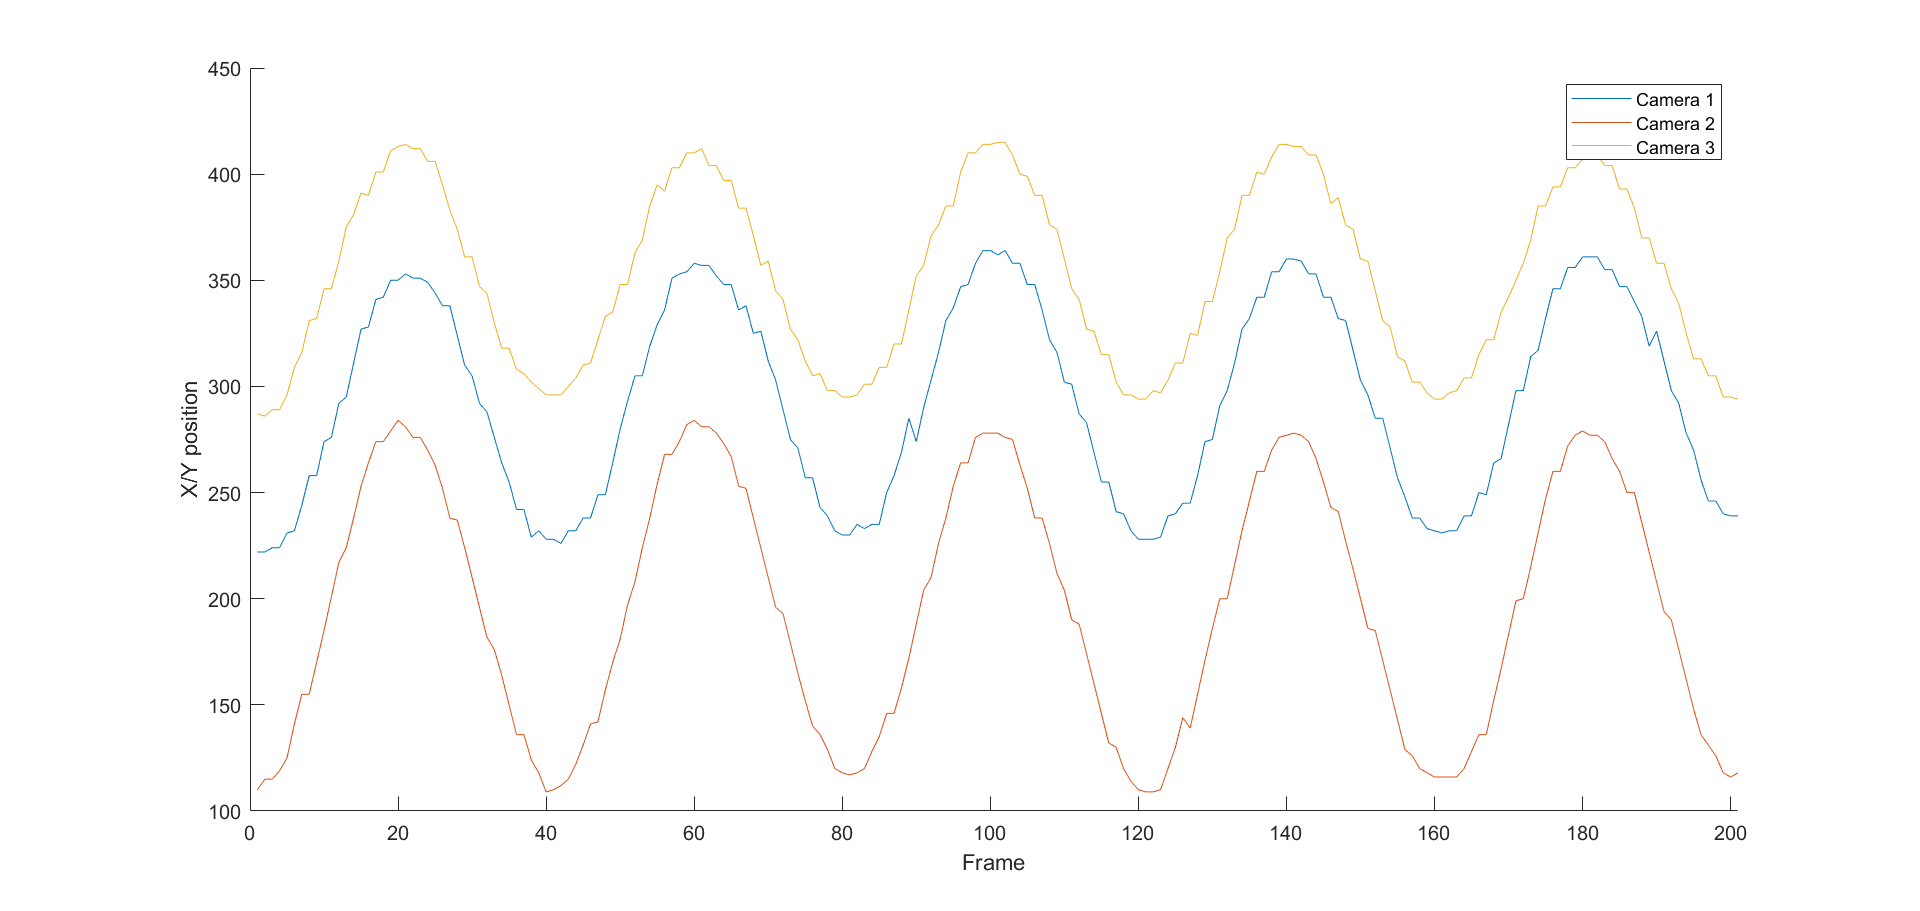
\includegraphics[scale=0.2]{./Figures/step1.png}
    \caption{Plots show the position of the object in the image row-space after synchronization and trimming of the dataset.}
  \label{fig:step1}
\end{figure}
\begin{figure}[!t]
  \centering
    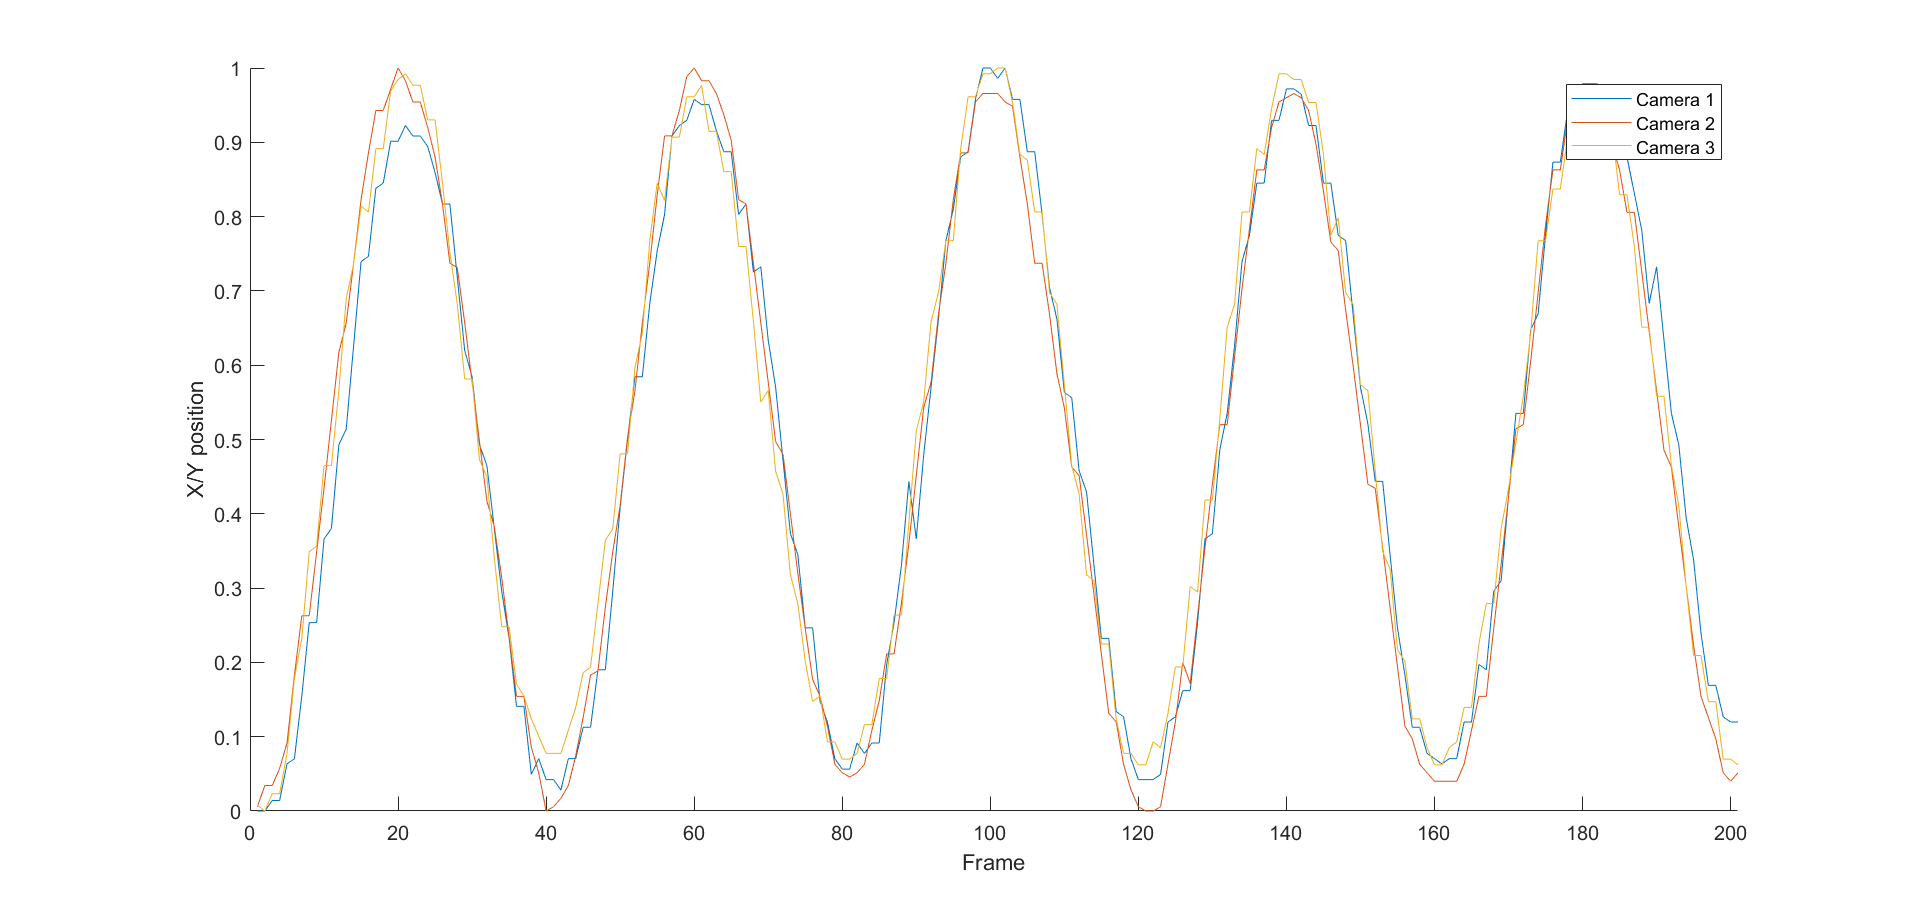
\includegraphics[scale=0.2]{./Figures/step2.png}
    \caption{Plots show the normalized position in the image row-space.}
  \label{fig:step2}
\end{figure}

The PCA was performed through SVD. The figure \ref{fig:test1}(a) shows the percentage of energy captured by each mode. The first three modes captured $\approx 90 \%$ of the total energy. In figure figure \ref{fig:test1}(b), the evolution of each linearly uncorrelated mode, obtained by projecting each data vector onto the left singular vector, was plotted. The first mode represents the simple harmomic motion of the object along $z$ direction. The second mode represents the change in the amplitude of oscillations. Other modes, with energy level $<10\%$, arise due to noise that comes from camera shake and error in position estimation.


\begin{figure}[!b]
\subfloat[Percentage of variance captured by each mode.]{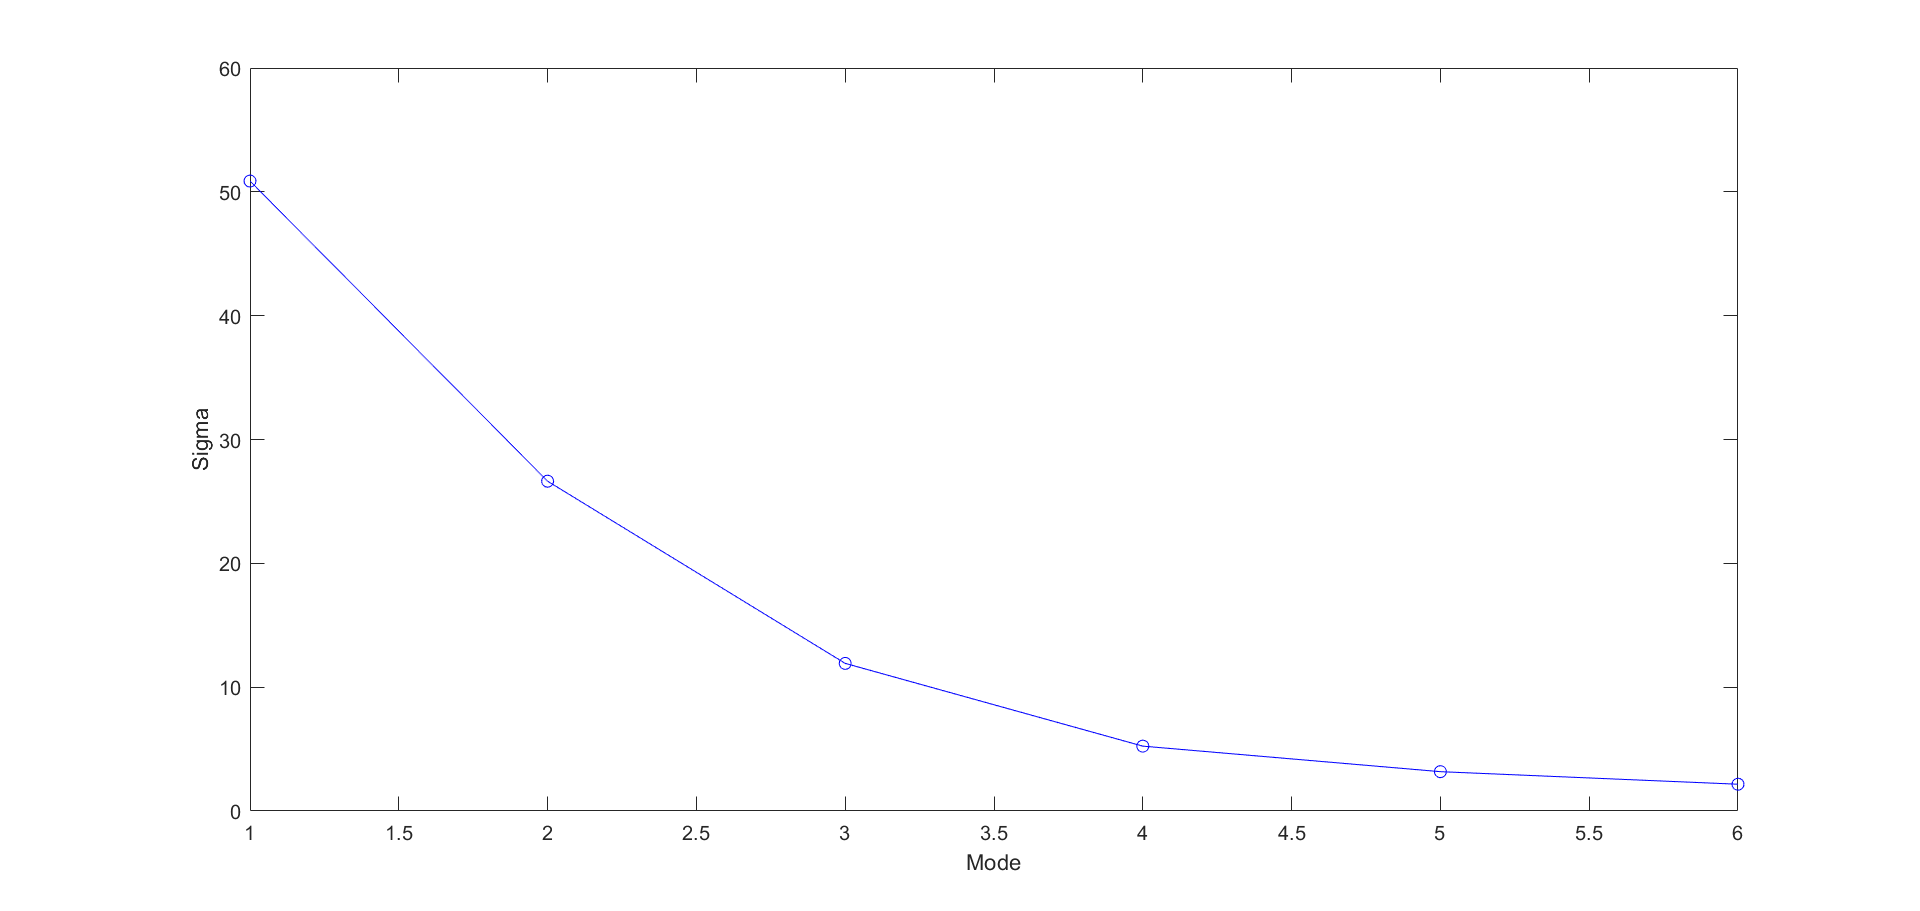
\includegraphics[width = 0.5\linewidth]{./Figures/test1_sigma.png}} 
\subfloat[Evolution of proper orthogonal modes.]{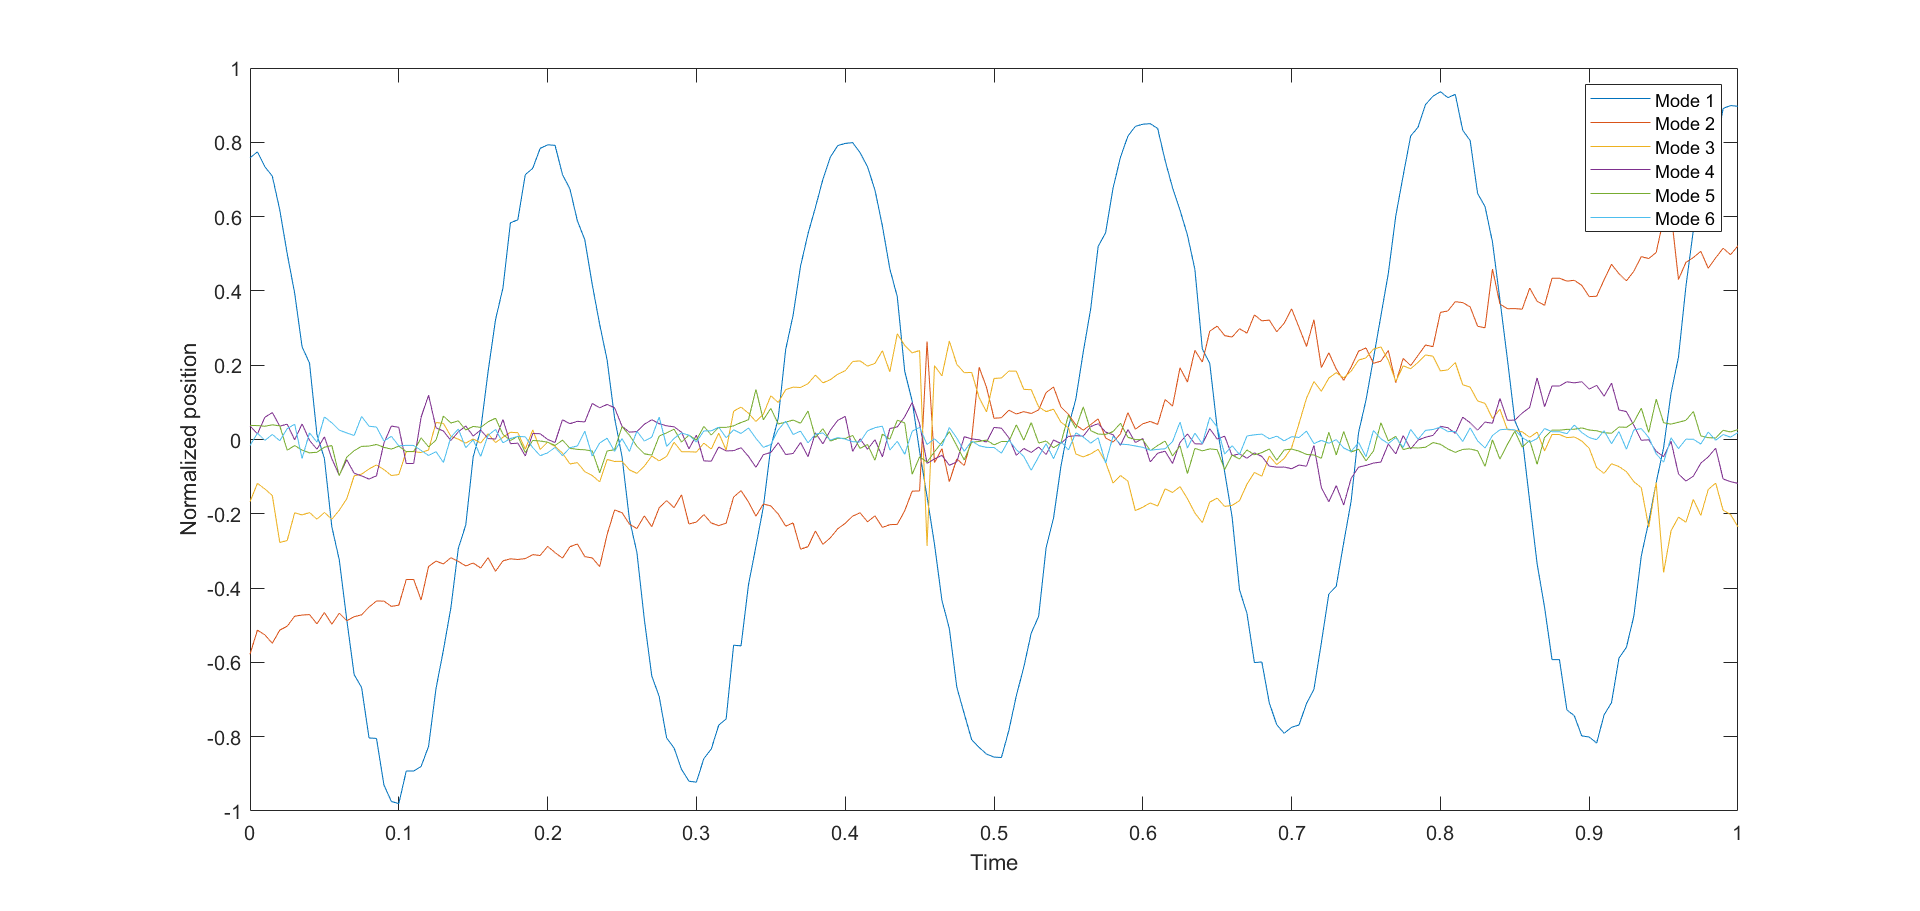
\includegraphics[width = 0.5\linewidth]{./Figures/test1_modes.png}}\\
\caption{Principal Component Analysis on dataset Test 1 through singular value decomposition.}
\label{fig:test1}
\end{figure}

\subsection{Test 2:}
In this test, the object was again moving in a simple harmonic motion along $z$ direction. However, large noise was injected into the datasets by shaking the camera. While the underlying dimension of the system was still $1$, it was observed that the PCA was not able to extract any feature from the data. The noise severly hampered the efficacy of the PCA. Figure \ref{fig:test2}(b) shows no distinct motion in any of the $6$ modes. 

\begin{figure}[!b]
\subfloat[Percentage of variance captured by each mode]{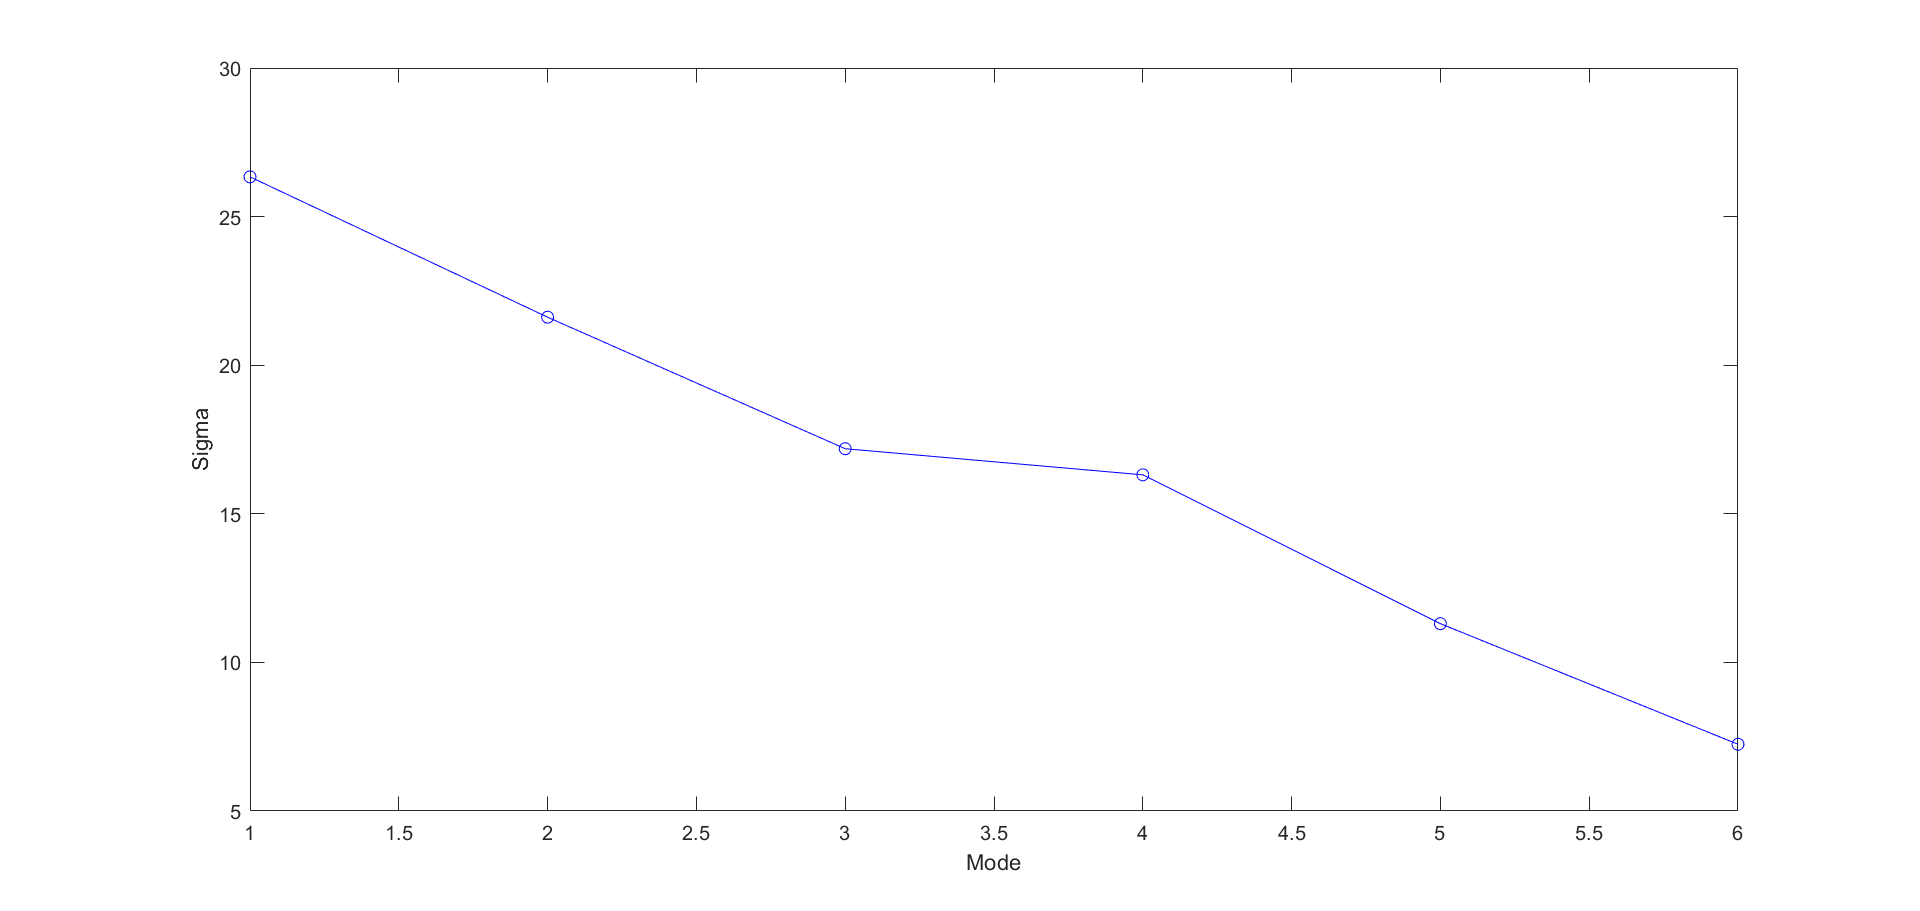
\includegraphics[width = 0.5\linewidth]{./Figures/test2_sigma.png}} 
\subfloat[Evolution of proper orthogonal modes.]{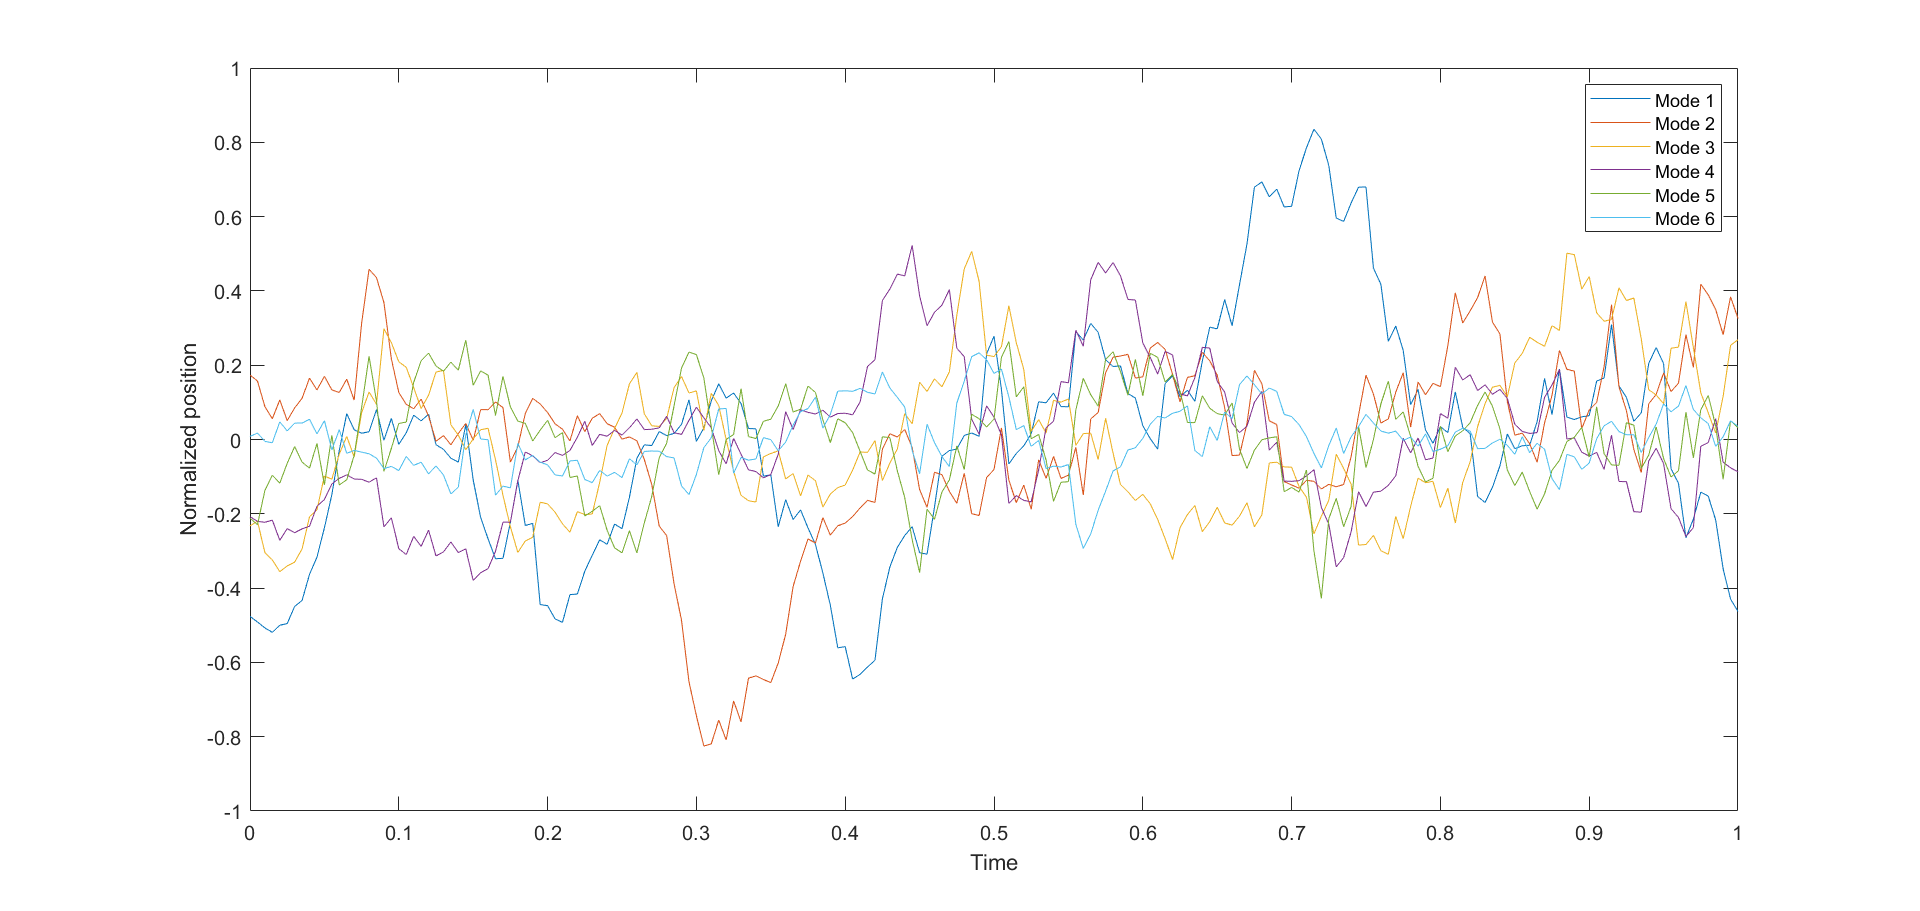
\includegraphics[width = 0.5\linewidth]{./Figures/test2_modes.png}}\\
\caption{Principal Component Analysis on dataset Test 2 through singular value decomposition.}
\label{fig:test2}
\end{figure}

\subsection{Test 3:}
In Test $3$ dataset, the object was moving in a simple harmonic motion along $z$ direction as well as in pendulum motion along $x$ and $y$ direction.  The noise level was relatively small (compared to Test $2$). The underlying system has $3$ degree of freedom. However, since we are estimation position through images, we are restricted to $2$D. Thus we expect PCA to be able to find $2$ principal modes to completely describe the motion in image space, given good position estimates are obtained. Unfortunately, the position estimtates were not as robust as that of Test $1$ because of the flashlight occlusion. On some part of the data, the position estimates drifted away from the true value. Therefore we see in the figure \ref{fig:test3}, $4$ dominant modes. Modes $1$ and $2$ represent the motion in the 2D image space, while modes $3$ and $4$ represent drift in the position estimates. Other modes correspond to the noise in the data.

\begin{figure}[!b]
\subfloat[Percentage of variance captured by each mode]{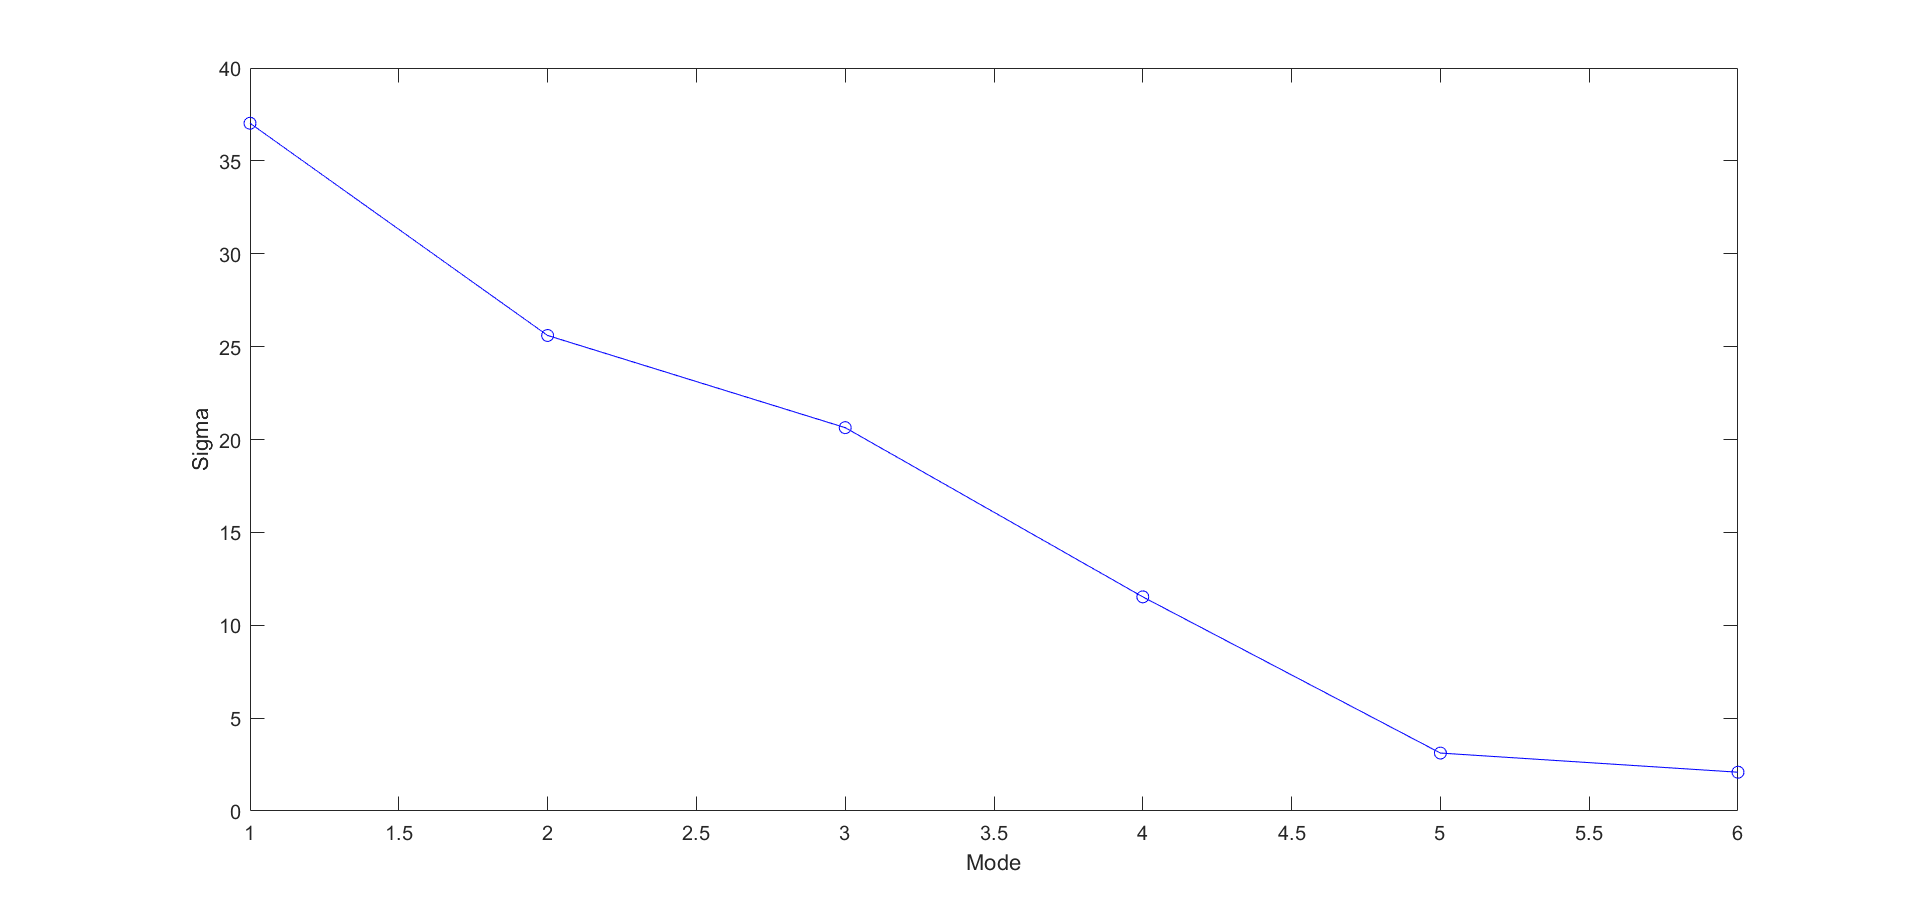
\includegraphics[width = 0.5\linewidth]{./Figures/test3_sigma.png}} 
\subfloat[Evolution of proper orthogonal modes.]{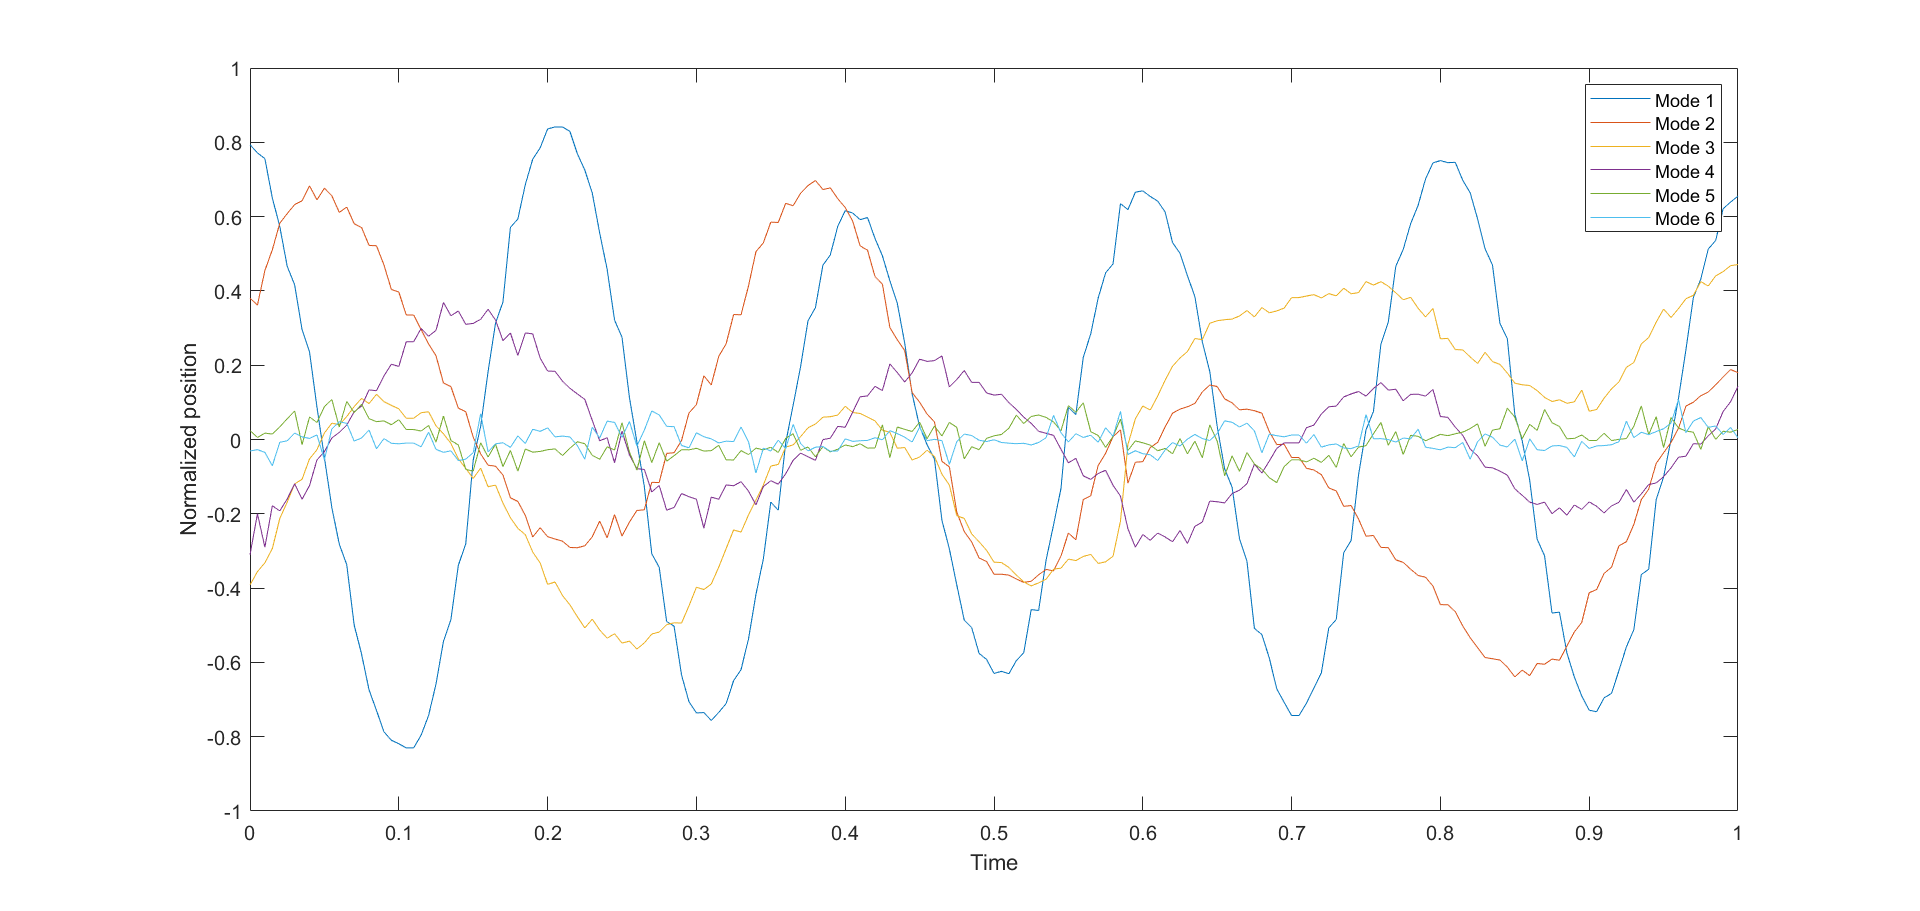
\includegraphics[width = 0.5\linewidth]{./Figures/test3_modes.png}}\\
\caption{Principal Component Analysis on dataset Test 3 through singular value decomposition.}
\label{fig:test3}
\end{figure}

\subsection{Test 4:}
In the last dataset, the object was moving in a simple harmonic motion along $z$ direction, in a pendulum motion along $x$ and $y$ direction and in a rotating motion about the $z$ axis. The noise level was again relatively small compared to Test $2$. In this case, the underlying dimension of the system is $4$. As mentioned earlier, since we are operating through images, PCA will at best give $2$ dominant modes. For this case, the object was tracked using a patch of white space in the paint. The rotation of flashlight made it difficult to track it. Thus, the data only captures $3$ degree of freedom motion, similar to Test $3$. The rotation of flashlight about $z$ axis is the latent variable that we do not expect to be resolved. Figure \ref{fig:test4}(b) shows two dominant modes that represents the simple harmonic motion along $z$ axis and the pendulum motion along $x$ and $y$ direction. Since the object's pendulum motion discipated quickly, we see same dissipation of mode $2$. Since, the noise in the position estimates was very large, we see large noisy modes.

\begin{figure}[!b]
\subfloat[Percentage of variance captured by each mode]{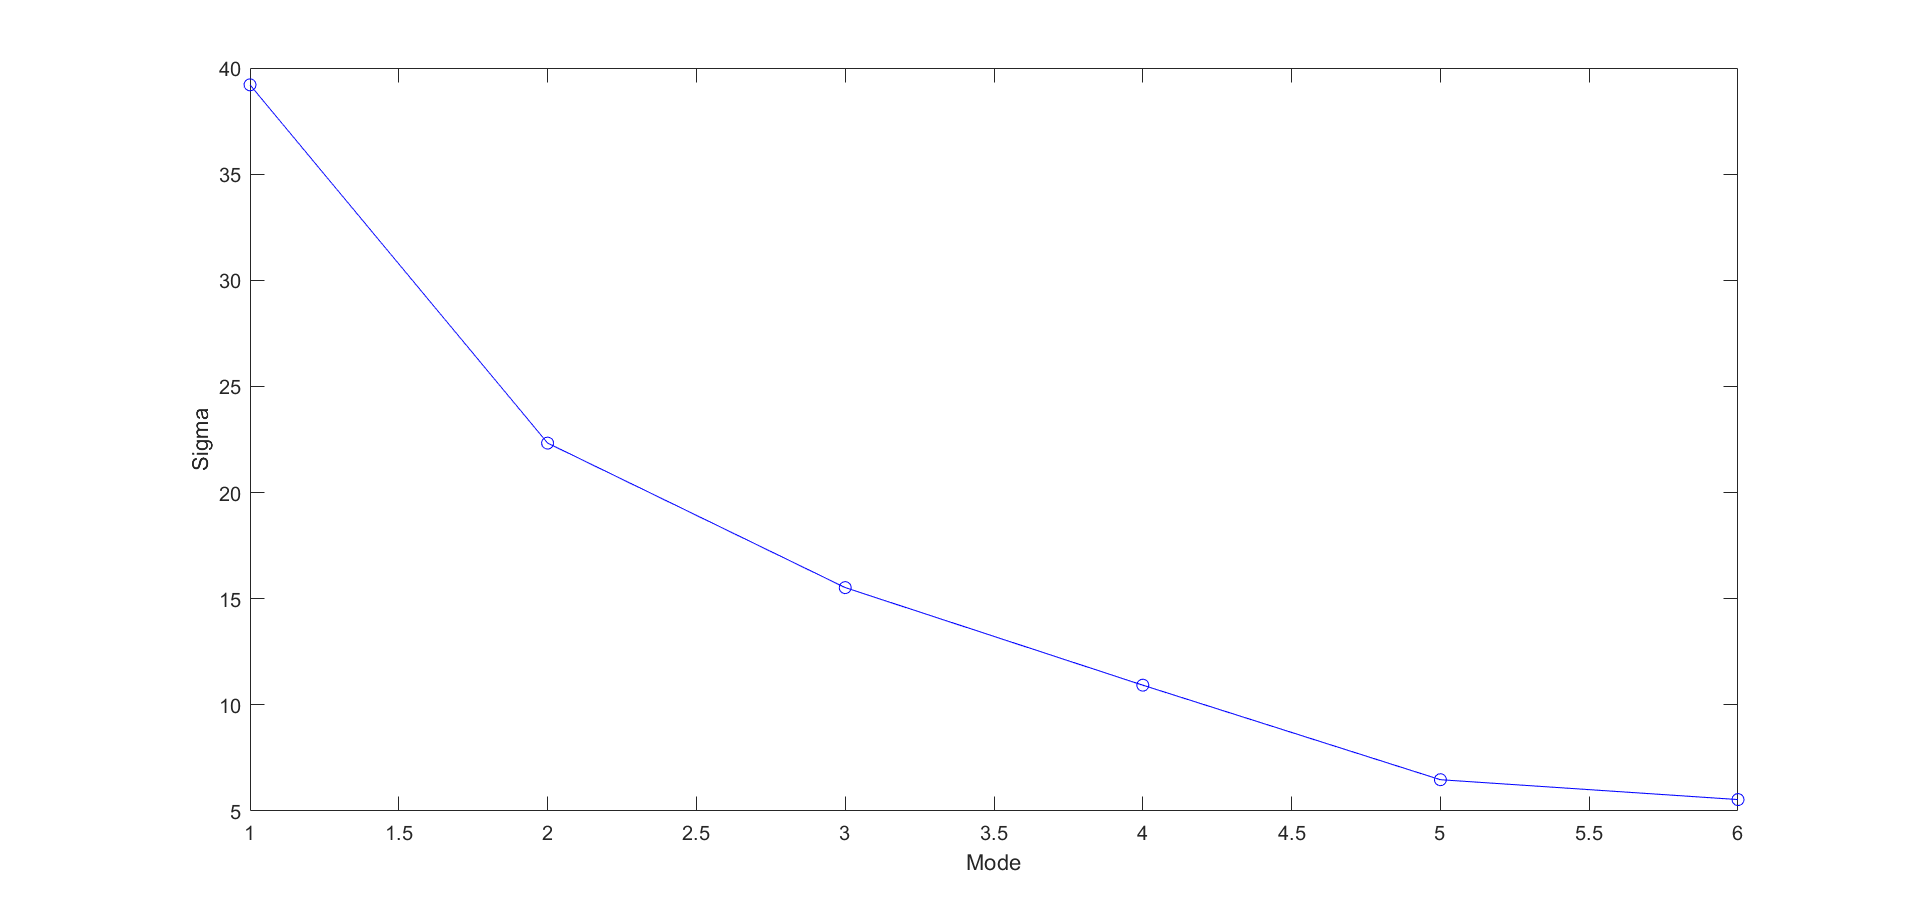
\includegraphics[width = 0.5\linewidth]{./Figures/test4_sigma.png}} 
\subfloat[Evolution of proper orthogonal modes.]{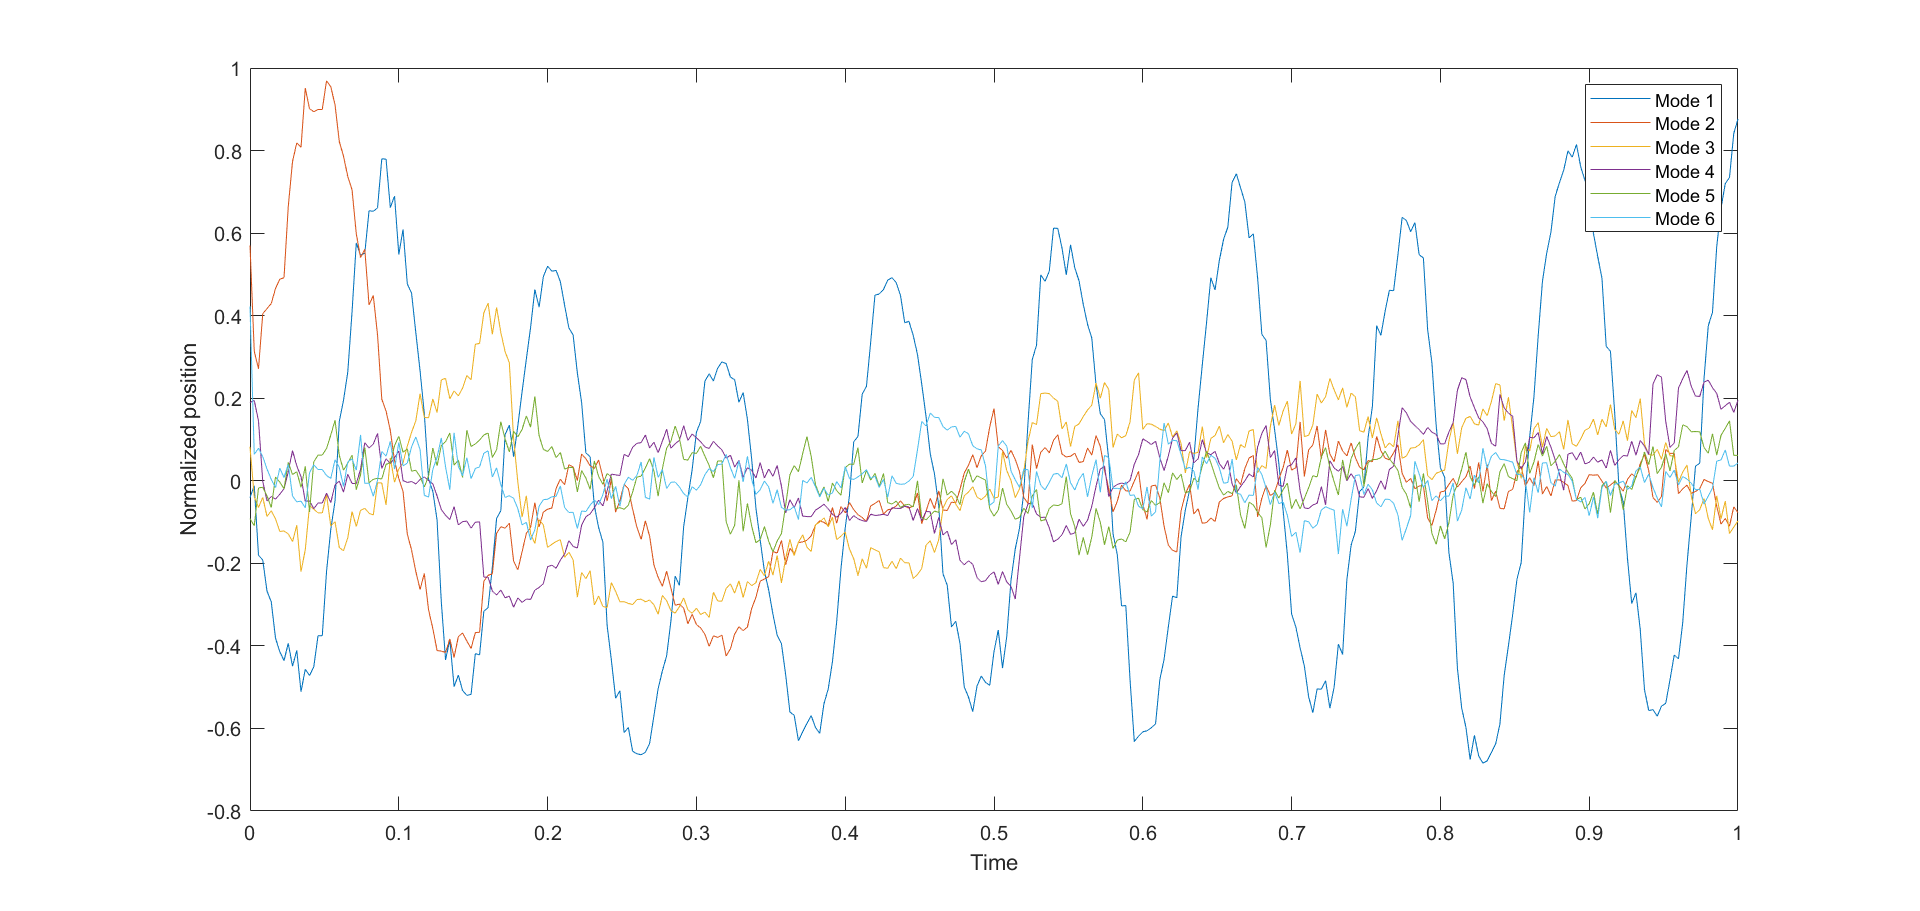
\includegraphics[width = 0.5\linewidth]{./Figures/test4_modes.png}}\\
\caption{Principal Component Analysis on dataset Test 4 through singular value decomposition.}
\label{fig:test4}
\end{figure}

\pagebreak
% Summary and Conclusions
\section{Summary and Conclusions}
The concept of reducing the dimensions of the dataset through diagonalization of the covariance matrix was introduced. PCA was used to extract the low-dimensional motion of the mass-string system from series of images. A tracking algorithm was written to estimate the position of the object in each frame. The positional data was then synchronized, trimmed and normalized for analysis. Each dataset was projected onto the left singular vectors obtained from the SVD to extract linearly uncorrelated modes (principal components). The effect of noise and the dimension of the feature space on the outcome of the PCA was also examined. It was found that large noise severely compromize the efficacy of PCA method. PCA was able to identify the simple harmonic motion of the object inTest $1$, $3$ and $4$. In Test $3$, it was able to also identify the pendulum motion of the object.

\pagebreak
% Appendices
\begin{appendices}

% MATLAB Functions
\section{MATLAB Functions}
Some important MATLAB functions used during the implementation.
\begin{itemize}
    \item \texttt{y = linspace(x1,x2,n)} returns a row vector of \texttt{n} evenly spaced points between \texttt{x1} and \texttt{x2}. 
    \item \texttt{ks = fftshift(k)} rearranges FT by shifting zero frequency component to the center of the array. Exchanges two halves of the array.
    \item \texttt{Y = fftn(X)} returns multidimensional Fourier transform of an N-D array using FFT algorithm.
    \item \texttt{[U,S,V] = svd(A)} performs a singular value decomposition of matrix A, such that A = U*S*V'.
    \item \texttt{B = repmat(A,r1,...,rN)} specifies a list of scalars, r1,..,rN, that describes how copies of A are arranged in each dimension. When A has N dimensions, the size of B is size(A).*[r1...rN]. For example, repmat([1 2; 3 4],2,3) returns a 4-by-6 matrix.
\end{itemize}

\pagebreak
% MATLAB Codes

\section{MATLAB Code}
\href{https://github.com/cssubedi/AMATH-582}{The code is published on the github repository AMATH-582 under Principal Component Analysis directory.} \\

\textbf{MATLAB code for extracting position.}
\lstinputlisting[style=Matlab-editor]{extract_position.m}
\pagebreak
\textbf{MATLAB code for PCA.}
\lstinputlisting[style=Matlab-editor]{principal_component_analysis.m}


\end{appendices}

\end{document}
